<<<<<<< HEAD
\documentclass{beamer}
\usepackage[utf8]{inputenc}
\usepackage{cite}
\usepackage{graphicx}
\usepackage{float}
\usepackage{fontawesome}
\usepackage{multicol}


% Beamer theme settings
\usetheme{CambridgeUS}
\usecolortheme{default}

\title{Semantic Textual Similarity}
\author{Bruno Sánchez Gómez and María del Carmen Ramírez Trujillo}
\date{\today}

\setbeamertemplate{footline}{%
    \leavevmode%
    \hbox{%
        \begin{beamercolorbox}[wd=0.6\paperwidth,ht=2.5ex,dp=1.125ex,center]{author in head/foot}%
            \hspace*{2mm}\insertshortauthor
        \end{beamercolorbox}%
        \begin{beamercolorbox}[wd=0.3\paperwidth,ht=2.5ex,dp=1.125ex,center]{title in head/foot}%
            \insertshorttitle
        \end{beamercolorbox}%
        \begin{beamercolorbox}[wd=0.1\paperwidth,ht=2.5ex,dp=1.125ex,center]{date in head/foot}%
            \hspace*{-2mm}\insertframenumber{} / \inserttotalframenumber
        \end{beamercolorbox}%
    }%
    \vskip0pt%
}

\begin{document}

\begin{frame}
    \titlepage
\end{frame}

\begin{frame}
    \frametitle{Table of Contents}
    \tableofcontents
\end{frame}

% Introduction
\section{Introduction}
\frame{\tableofcontents[currentsection]}
\begin{frame}{Introduction}
    \begin{itemize}
        \item {\large Based on the data and evaluation frameworks for \textit{SemEval-2012 Task 6: A Pilot on Semantic Textual
         Similarity,} propose a framework to evaluate semantic similarity between pairs of sentences.}
    \end{itemize}
\end{frame}

\section{Methodology}
\frame{\tableofcontents[currentsection]}

\begin{frame}{Methodology overview}
    \begin{itemize}
        \item Feature extraction:
        \begin{itemize}
            \item Syntactic features (8)
            \item Lexical features (32)
            \item String features (18)
        \end{itemize}
        \vspace{0.4cm}
        \item Preprocessing: remove punctuation and convert to lower case.
        \begin{itemize}
            \item Extra preprocessing (for lexical and string feature extraction):
            \begin{itemize}
                \item Stop words
                \item Lemmatization
                \item Word sense disambiguation
            \end{itemize}
        \end{itemize}
        \vspace{0.4cm}
        \item Training models:
        \begin{itemize}
            \item Multi-Layer Perceptron (MLP)
            \item Support Vector Regressor (SVR)
            \item Random Forest Regressor (RFR)
        \end{itemize} 
    \end{itemize}
\end{frame}

\begin{frame}{Syntactic Features}
    \textit{Process of analyzing a sentence's structure according to the grammatical rules and how words are related withing 
    the sentence.}
    \vspace{1cm}
    \begin{itemize}
        \item N-grams overlap removing function words (prepositions, conjunctions, articles)
    \end{itemize}
    \vspace{1cm}
    Sentence: "a horse eats carrots" $\Rightarrow$ "horse eats carrots" (content words)
         \[ ngo(S_1, S_2) = 2 \cdot \left( \frac{|S_1|}{|S_1 \cap S_2|} + \frac{|S_2|}{|S_1 \cap S_2|} \right)^{-1} \]
\end{frame}

\begin{frame}{Syntactic Features}
    \begin{itemize}
        \item Syntactic roles similarity 
    \end{itemize}
    \vspace{0.3cm}
    \texttt{python library Stanza} (Stanford NLP Group, 2006)\\ \vspace{0.1cm}
    Sentence: "a horse eats carrots and the man cleans the farm for the owner" \\ \vspace{0.1cm}
    \texttt{'p': [\{'carrot','eat'\}, \{'owner','farm','for','clean'\}],
    \\ 's': [\{'horse'\}, \{'man'\}], 
    \\ 'o': [\{'carrot'\}, \{'farm'\}, \{'for', 'owner'\}]}
         \[ chunksim(C1, C2) = \sum_{ l_1 \in C1} \sum_{l_2 \in C2}  ssim(l_1, l_2) \]
\end{frame}

\begin{frame}{Syntactic Features}
    \begin{itemize}
        \item Syntactic dependencies overlap
    \end{itemize}
    \vspace{0.2cm}
    \texttt{python library Stanza} (Stanford NLP Group, 2006) \\
    Sentence: "a horse eats carrots" \\
    \begin{center}
        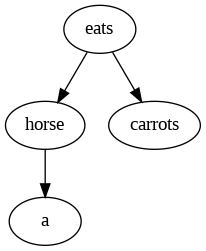
\includegraphics[width=0.22\textwidth]{figures/dependency_tree.png}
    \end{center}
        \[ \text{wdrc}(S_1, S_2) = \frac{\sum_{r \in S_1 \cap S_2} \max(\text{ic}(g(r)), \text{ic}(d(r)))}{\sum_{r \in S_2} 
\max(\text{ic}(g(r)), \text{ic}(d(r)))} \]
\end{frame}

\begin{frame}{Lexical features}
\textit{The process of analyzing a sentence's structure through the identification and classification of individual words.}
\vspace{0.5cm}
\begin{itemize}
    \item Jaccard distance 
    \item Containtment similarity 
    \item Lin similarity 
    \item Resnik similarity 
    \item WordNet augmented word overlap 
    \item Weighted word overlap 
    \item Greedy lemma aligning overlap
\end{itemize}
\end{frame}

\begin{frame}{Lexical features}
    \textit{The process of analyzing a sentence's structure through the identification and classification of individual words.}
    \vspace{0.5cm}
    \begin{itemize}
        \item Jaccard distance 
        \item \textbf{Containtment similarity}
        \item Lin similarity 
        \item \textbf{Resnik similarity }
        \item \textbf{Weighted word overlap}
        \item \textbf{WordNet augmented word overlap}
        \item \textbf{Greedy lemma aligning overlap}
    \end{itemize}
\end{frame}

    \begin{frame}{Lexical features}
        The sets $S_1$ and $S_2$ will be list of words or n-tuples of n-grams of each sentence. \\
        \begin{itemize}
            \item Containtment similarity measure (Broder, 1997)
            \[
            csimm(S_1,S_2) = \frac{\left| S_1 \cap S_2 \right|}{\min \{ \left| S_1 \right|, \left| S_2 \right| \}}
            \]
            \item Resnik similarity 
            \[resniksim(S_1,S_2) = ic(LCS(S_1,S_2)) \]
            \item Weighted word overlap 
            \[
            wwc(S_1, S_2) = 
            \frac{\sum_{w \in S_1 \cap S_2} ic(w)}{\sum_{w' \in S_2} ic(w')}
            \]
        \end{itemize}
\end{frame}

\begin{frame}{Lexical features}
    \begin{itemize}
    \item WordNet augmented word overlap 
    \[ P_{WN}(S_1, S_2) = \frac{1}{|S_2|} \sum_{w_1 \in S_1} \text{score}(w_1, S_2)\]
    \[
    \text{score}(w, S) = 
    \begin{cases} 
    1 & \text{if } w \in S \\ 
    \max_{w' \in S} \{\text{pathsim}(w, w')\} & \text{otherwise}
    \end{cases}
    \]
    \vspace{0.3cm}
\item Greedy lemma aligning overlap
    \[ glao(S_1, S_2) = \frac{\sum_{(l_1, l_2) \in P} \max \{ \text{ic}(l_1), \text{ic}(l_2) \} \cdot \text{linsim}(l_1, l_2)}{\max \{|S_1|, |S_2|\}} \]
    P is the set of lemma pairs obtained by greedy alignment.
\end{itemize}
\end{frame}

\begin{frame}{String Feature}

    \begin{itemize}
        \item Character n-grams (Barrón-Cedeño, 2010)
        \vspace{0.2cm}
        \begin{itemize}
            \item \texttt{from sklearn.feature\_extraction.text import TfidfVectorizer} 
        \end{itemize}
        \vspace{0.2cm} 
        Sentece: "a horse eats carrots" \\ \vspace{0.2cm}
        3-grams strigns: ['a h', ' ho', 'hor', 'ors', 'rse', 'se ', 'e e', ' ea', 'eat', 'ats', 'ts ', 's c', ' ca', 'car', 'arr', 'rro', 'rot', 'ots']
        \[ 
            \text{cossim(A,B)} = \frac{\mathbf{A} \cdot \mathbf{B}}{\|\mathbf{A}\| \|\mathbf{B}\|}
             \]
    \end{itemize}

    \begin{itemize}
        \item Greedy String Tailing
    \end{itemize}
    \[
gstsim(S_1, S_2) = \frac{\sum_{t \in S_1 \cap S_2} \text{len}(t)}{\max \{ \text{len}(S_1), \text{len}(S_2) \}}
\]
        Threshold for the lenght of the tile: 5, 10. \\ \vspace{0.1cm}
\end{frame}

\begin{frame}{Model training and testing}
    \begin{itemize}
        \item Multi-Layer Perceptron (MLP)
        \item Support Vector Regressor (SVR)
        \item Random Forest Regressor (RFR)
    \end{itemize} 
    \vspace{1cm}
    \begin{itemize}
        \item Feature selection: 10 features with the highest absolute pearson correlation with gs.
    \end{itemize}

\end{frame}

 % mari
\section{Results}
\frame{\tableofcontents[currentsection]}

\begin{frame}
    \frametitle{Model \& Feature Overview}
    \begin{itemize}
      \item Models: MLP, SVR, RFR.
      \item Features: 
      \begin{itemize}
        \item Lexical, Syntactic, Strings (individually).
        \item Unrestricted (Lexical + Syntactic + Strings).
        \item FeatureSelection, based on:
        \begin{itemize}
            \item Pearson correlation for MLP/SVR
            \item Feature importance for RFR
        \end{itemize}
      \end{itemize}
      \item Performance measured using Pearson correlation with the Gold Standard
    \end{itemize}
\end{frame}
    

\begin{frame}
    \frametitle{Results Summary}
    \begin{table}[ht]
        \centering
        \begin{tabular}{|l|c|c|c|}
            \hline
            \textbf{Features} & \textbf{MLP} & \textbf{SVR} & \textbf{RFR} \\
            \hline
            Lexical            & 0.607       & 0.681       & 0.728 \\
            Syntactic          & 0.666       & 0.658       & 0.661 \\
            Strings            & 0.674       & 0.676       & 0.685 \\
            Unrestricted       & 0.652       & 0.744       & \textbf{0.757} \\
            FeatureSelection   & 0.744       & 0.742       & 0.745 \\
            \hline
        \end{tabular}
    \end{table}
    \begin{itemize}
      \item Best performance: RFR with Unrestricted (0.757)
      \item Syntactic features less informative than Lexical/Strings
      \item Feature combination improves SVR/RFR
      \item MLP suffers from overfitting
    \end{itemize}
\end{frame}
    

\begin{frame}
    \frametitle{Top Features: Pearson Correlation}
    Top 5 features based on Pearson correlation with the Gold Standard:
  
    \begin{table}[ht]
      \centering
      \begin{tabular}{|l|c|}
        \hline
        \textbf{Feature} & \textbf{Correlation} \\
        \hline
        lemmas\_wn\_aug\_overlap & 0.7233 \\
        normal\_char\_2gram & 0.7216 \\
        lemmas\_char\_2gram & 0.6902 \\
        sw\_char\_2gram & 0.6876 \\
        sw\_gst\_5 & 0.6666 \\
        \hline
      \end{tabular}
    \end{table}
  
    Three key feature types:
    \begin{itemize}
      \item WordNet-Augmented Overlap (Lexical)
      \item Character n-grams (String-based)
      \item Greedy String Tiling (String-based)
    \end{itemize}
\end{frame}

\begin{frame}
    \frametitle{Top Features: Feature Importance}
    Top 5 features based on Feature Importance scores from RFR:
  
    \begin{table}[ht]
      \centering
      \begin{tabular}{|l|c|}
        \hline
        \textbf{Feature} & \textbf{Importance} \\
        \hline
        lemmas\_wn\_aug\_overlap & 0.4325 \\
        normal\_char\_2gram & 0.1630 \\
        chunk\_sim\_s & 0.0413 \\
        lemmas\_weighted\_overlap & 0.0275 \\
        normal\_char\_5gram & 0.0199 \\
        \hline
      \end{tabular}
    \end{table}
  
    The top 2 features:
    \begin{itemize}
      \item Common with Pearson correlation table.
      \item Have significantly higher importance, indicating their dominance in sentence similarity prediction
    \end{itemize}
    
    Feature types: 2 Lexical, 1 Syntactic, 2 Strings-related.
\end{frame} % bruno
\section{Conclusion}
\frame{\tableofcontents[currentsection]}

\begin{frame}
    \frametitle{Conclusion}
    \begin{itemize}
        \item Best performance: RFR with Unrestricted features (0.757 Pearson correlation).
        \item Key features: \textit{WordNet-Augmented Overlap} and \textit{Character n-grams}.
        \item Lexical and String-based features encode most of the relevant information for STS.
        \item Combining feature types (Lexical, Syntactic, Strings) significantly boosts performance.
    \end{itemize}
\end{frame}

% References
\begin{frame}{References}
    \begin{itemize}
        \item Agirre, Eneko, Daniel Cer, Mona Diab, and Aitor Gonzalez-Agirre. (2012) "SemEval-2012 Task 6: A Pilot on Semantic Textual Similarity." SEM 2012. 385-393. 
        \item D. Bär, C. Biemann, I. Gurevych and T. Zesch. (2012). UKP: Computing Semantic Textual Similarity by Combining Multiple Content Similarity Measures. 435-440. 
        \item F. Sari, G. Glavaš, M. Karan, J. Snajder, B. Dalbelo Bašić. (2012). TakeLab: Systems for Measuring Semantic Text Similarity. Proceedings of SemEval-2012. 
    \end{itemize}    
\end{frame}

=======
\documentclass{beamer}
\usepackage[utf8]{inputenc}
\usepackage{cite}
\usepackage{graphicx}
\usepackage{float}
\usepackage{fontawesome}
\usepackage{multicol}


% Beamer theme settings
\usetheme{CambridgeUS}
\usecolortheme{default}

\title{Semantic Textual Similarity}
\author{Bruno Sánchez Gómez and María del Carmen Ramírez Trujillo}
\date{\today}

\setbeamertemplate{footline}{%
    \leavevmode%
    \hbox{%
        \begin{beamercolorbox}[wd=0.6\paperwidth,ht=2.5ex,dp=1.125ex,center]{author in head/foot}%
            \hspace*{2mm}\insertshortauthor
        \end{beamercolorbox}%
        \begin{beamercolorbox}[wd=0.3\paperwidth,ht=2.5ex,dp=1.125ex,center]{title in head/foot}%
            \insertshorttitle
        \end{beamercolorbox}%
        \begin{beamercolorbox}[wd=0.1\paperwidth,ht=2.5ex,dp=1.125ex,center]{date in head/foot}%
            \hspace*{-2mm}\insertframenumber{} / \inserttotalframenumber
        \end{beamercolorbox}%
    }%
    \vskip0pt%
}

\begin{document}

\begin{frame}
    \titlepage
\end{frame}

\begin{frame}
    \frametitle{Table of Contents}
    \tableofcontents
\end{frame}

% Introduction
\section{Introduction}
\frame{\tableofcontents[currentsection]}
\begin{frame}{Introduction}
    \begin{itemize}
        \item {\large Based on the data and evaluation frameworks for \textit{SemEval-2012 Task 6: A Pilot on Semantic Textual
         Similarity,} propose a framework to evaluate semantic similarity between pairs of sentences.}
    \end{itemize}
\end{frame}

\section{Methodology}
\frame{\tableofcontents[currentsection]}

\begin{frame}{Methodology overview}
    \begin{itemize}
        \item Feature extraction:
        \begin{itemize}
            \item Syntactic features (8)
            \item Lexical features (32)
            \item String features (18)
        \end{itemize}
        \vspace{0.4cm}
        \item Preprocessing: remove punctuation and convert to lower case.
        \begin{itemize}
            \item Extra preprocessing (for lexical and string feature extraction):
            \begin{itemize}
                \item Stop words
                \item Lemmatization
                \item Word sense disambiguation
            \end{itemize}
        \end{itemize}
        \vspace{0.4cm}
        \item Training models:
        \begin{itemize}
            \item Multi-Layer Perceptron (MLP)
            \item Support Vector Regressor (SVR)
            \item Random Forest Regressor (RFR)
        \end{itemize} 
    \end{itemize}
\end{frame}

\begin{frame}{Syntactic Features}
    \textit{Process of analyzing a sentence's structure according to the grammatical rules and how words are related withing 
    the sentence.}
    \vspace{1cm}
    \begin{itemize}
        \item N-grams overlap removing function words (prepositions, conjunctions, articles)
    \end{itemize}
    \vspace{1cm}
    Sentence: "a horse eats carrots" $\Rightarrow$ "horse eats carrots" (content words)
         \[ ngo(S_1, S_2) = 2 \cdot \left( \frac{|S_1|}{|S_1 \cap S_2|} + \frac{|S_2|}{|S_1 \cap S_2|} \right)^{-1} \]
\end{frame}

\begin{frame}{Syntactic Features}
    \begin{itemize}
        \item Syntactic roles similarity 
    \end{itemize}
    \vspace{0.3cm}
    \texttt{python library Stanza} (Stanford NLP Group, 2006)\\ \vspace{0.1cm}
    Sentence: "a horse eats carrots and the man cleans the farm for the owner" \\ \vspace{0.1cm}
    \texttt{'p': [\{'carrot','eat'\}, \{'owner','farm','for','clean'\}],
    \\ 's': [\{'horse'\}, \{'man'\}], 
    \\ 'o': [\{'carrot'\}, \{'farm'\}, \{'for', 'owner'\}]}
         \[ chunksim(C1, C2) = \sum_{ l_1 \in C1} \sum_{l_2 \in C2}  ssim(l_1, l_2) \]
\end{frame}

\begin{frame}{Syntactic Features}
    \begin{itemize}
        \item Syntactic dependencies overlap
    \end{itemize}
    \vspace{0.2cm}
    \texttt{python library Stanza} (Stanford NLP Group, 2006) \\
    Sentence: "a horse eats carrots" \\
    \begin{center}
        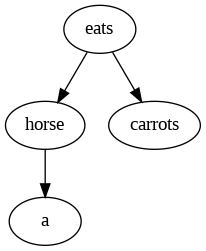
\includegraphics[width=0.22\textwidth]{figures/dependency_tree.png}
    \end{center}
        \[ \text{wdrc}(S_1, S_2) = \frac{\sum_{r \in S_1 \cap S_2} \max(\text{ic}(g(r)), \text{ic}(d(r)))}{\sum_{r \in S_2} 
\max(\text{ic}(g(r)), \text{ic}(d(r)))} \]
\end{frame}

\begin{frame}{Lexical features}
\textit{The process of analyzing a sentence's structure through the identification and classification of individual words.}
\vspace{0.5cm}
\begin{itemize}
    \item Jaccard distance 
    \item Containtment similarity 
    \item Lin similarity 
    \item Resnik similarity 
    \item WordNet augmented word overlap 
    \item Weighted word overlap 
    \item Greedy lemma aligning overlap
\end{itemize}
\end{frame}

\begin{frame}{Lexical features}
    \textit{The process of analyzing a sentence's structure through the identification and classification of individual words.}
    \vspace{0.5cm}
    \begin{itemize}
        \item Jaccard distance 
        \item \textbf{Containtment similarity}
        \item Lin similarity 
        \item \textbf{Resnik similarity }
        \item \textbf{Weighted word overlap}
        \item \textbf{WordNet augmented word overlap}
        \item \textbf{Greedy lemma aligning overlap}
    \end{itemize}
\end{frame}

    \begin{frame}{Lexical features}
        The sets $S_1$ and $S_2$ will be list of words or n-tuples of n-grams of each sentence. \\
        \begin{itemize}
            \item Containtment similarity measure (Broder, 1997)
            \[
            csimm(S_1,S_2) = \frac{\left| S_1 \cap S_2 \right|}{\min \{ \left| S_1 \right|, \left| S_2 \right| \}}
            \]
            \item Resnik similarity 
            \[resniksim(S_1,S_2) = ic(LCS(S_1,S_2)) \]
            \item Weighted word overlap 
            \[
            wwc(S_1, S_2) = 
            \frac{\sum_{w \in S_1 \cap S_2} ic(w)}{\sum_{w' \in S_2} ic(w')}
            \]
        \end{itemize}
\end{frame}

\begin{frame}{Lexical features}
    \begin{itemize}
    \item WordNet augmented word overlap 
    \[ P_{WN}(S_1, S_2) = \frac{1}{|S_2|} \sum_{w_1 \in S_1} \text{score}(w_1, S_2)\]
    \[
    \text{score}(w, S) = 
    \begin{cases} 
    1 & \text{if } w \in S \\ 
    \max_{w' \in S} \{\text{pathsim}(w, w')\} & \text{otherwise}
    \end{cases}
    \]
    \vspace{0.3cm}
\item Greedy lemma aligning overlap
    \[ glao(S_1, S_2) = \frac{\sum_{(l_1, l_2) \in P} \max \{ \text{ic}(l_1), \text{ic}(l_2) \} \cdot \text{linsim}(l_1, l_2)}{\max \{|S_1|, |S_2|\}} \]
    P is the set of lemma pairs obtained by greedy alignment.
\end{itemize}
\end{frame}

\begin{frame}{String Feature}

    \begin{itemize}
        \item Character n-grams (Barrón-Cedeño, 2010)
        \vspace{0.2cm}
        \begin{itemize}
            \item \texttt{from sklearn.feature\_extraction.text import TfidfVectorizer} 
        \end{itemize}
        \vspace{0.2cm} 
        Sentece: "a horse eats carrots" \\ \vspace{0.2cm}
        3-grams strigns: ['a h', ' ho', 'hor', 'ors', 'rse', 'se ', 'e e', ' ea', 'eat', 'ats', 'ts ', 's c', ' ca', 'car', 'arr', 'rro', 'rot', 'ots']
        \[ 
            \text{cossim(A,B)} = \frac{\mathbf{A} \cdot \mathbf{B}}{\|\mathbf{A}\| \|\mathbf{B}\|}
             \]
    \end{itemize}

    \begin{itemize}
        \item Greedy String Tailing
    \end{itemize}
    \[
gstsim(S_1, S_2) = \frac{\sum_{t \in S_1 \cap S_2} \text{len}(t)}{\max \{ \text{len}(S_1), \text{len}(S_2) \}}
\]
        Threshold for the lenght of the tile: 5, 10. \\ \vspace{0.1cm}
\end{frame}

\begin{frame}{Model training and testing}
    \begin{itemize}
        \item Multi-Layer Perceptron (MLP)
        \item Support Vector Regressor (SVR)
        \item Random Forest Regressor (RFR)
    \end{itemize} 
    \vspace{1cm}
    \begin{itemize}
        \item Feature selection: 10 features with the highest absolute pearson correlation with gs.
    \end{itemize}

\end{frame}

 % mari
\section{Results}
\frame{\tableofcontents[currentsection]}

\begin{frame}
    \frametitle{Model \& Feature Overview}
    \begin{itemize}
      \item Models: MLP, SVR, RFR.
      \item Features: 
      \begin{itemize}
        \item Lexical, Syntactic, Strings (individually).
        \item Unrestricted (Lexical + Syntactic + Strings).
        \item FeatureSelection, based on:
        \begin{itemize}
            \item Pearson correlation for MLP/SVR
            \item Feature importance for RFR
        \end{itemize}
      \end{itemize}
      \item Performance measured using Pearson correlation with the Gold Standard
    \end{itemize}
\end{frame}
    

\begin{frame}
    \frametitle{Results Summary}
    \begin{table}[ht]
        \centering
        \begin{tabular}{|l|c|c|c|}
            \hline
            \textbf{Features} & \textbf{MLP} & \textbf{SVR} & \textbf{RFR} \\
            \hline
            Lexical            & 0.607       & 0.681       & 0.728 \\
            Syntactic          & 0.666       & 0.658       & 0.661 \\
            Strings            & 0.674       & 0.676       & 0.685 \\
            Unrestricted       & 0.652       & 0.744       & \textbf{0.757} \\
            FeatureSelection   & 0.744       & 0.742       & 0.745 \\
            \hline
        \end{tabular}
    \end{table}
    \begin{itemize}
      \item Best performance: RFR with Unrestricted (0.757)
      \item Syntactic features less informative than Lexical/Strings
      \item Feature combination improves SVR/RFR
      \item MLP suffers from overfitting
    \end{itemize}
\end{frame}
    

\begin{frame}
    \frametitle{Top Features: Pearson Correlation}
    Top 5 features based on Pearson correlation with the Gold Standard:
  
    \begin{table}[ht]
      \centering
      \begin{tabular}{|l|c|}
        \hline
        \textbf{Feature} & \textbf{Correlation} \\
        \hline
        lemmas\_wn\_aug\_overlap & 0.7233 \\
        normal\_char\_2gram & 0.7216 \\
        lemmas\_char\_2gram & 0.6902 \\
        sw\_char\_2gram & 0.6876 \\
        sw\_gst\_5 & 0.6666 \\
        \hline
      \end{tabular}
    \end{table}
  
    Three key feature types:
    \begin{itemize}
      \item WordNet-Augmented Overlap (Lexical)
      \item Character n-grams (String-based)
      \item Greedy String Tiling (String-based)
    \end{itemize}
\end{frame}

\begin{frame}
    \frametitle{Top Features: Feature Importance}
    Top 5 features based on Feature Importance scores from RFR:
  
    \begin{table}[ht]
      \centering
      \begin{tabular}{|l|c|}
        \hline
        \textbf{Feature} & \textbf{Importance} \\
        \hline
        lemmas\_wn\_aug\_overlap & 0.4325 \\
        normal\_char\_2gram & 0.1630 \\
        chunk\_sim\_s & 0.0413 \\
        lemmas\_weighted\_overlap & 0.0275 \\
        normal\_char\_5gram & 0.0199 \\
        \hline
      \end{tabular}
    \end{table}
  
    The top 2 features:
    \begin{itemize}
      \item Common with Pearson correlation table.
      \item Have significantly higher importance, indicating their dominance in sentence similarity prediction
    \end{itemize}
    
    Feature types: 2 Lexical, 1 Syntactic, 2 Strings-related.
\end{frame} % bruno
\section{Conclusion}
\frame{\tableofcontents[currentsection]}

\begin{frame}
    \frametitle{Conclusion}
    \begin{itemize}
        \item Best performance: RFR with Unrestricted features (0.757 Pearson correlation).
        \item Key features: \textit{WordNet-Augmented Overlap} and \textit{Character n-grams}.
        \item Lexical and String-based features encode most of the relevant information for STS.
        \item Combining feature types (Lexical, Syntactic, Strings) significantly boosts performance.
    \end{itemize}
\end{frame}

% References
\begin{frame}{References}
    \begin{itemize}
        \item Agirre, Eneko, Daniel Cer, Mona Diab, and Aitor Gonzalez-Agirre. (2012) "SemEval-2012 Task 6: A Pilot on Semantic Textual Similarity." SEM 2012. 385-393. 
        \item D. Bär, C. Biemann, I. Gurevych and T. Zesch. (2012). UKP: Computing Semantic Textual Similarity by Combining Multiple Content Similarity Measures. 435-440. 
        \item F. Sari, G. Glavaš, M. Karan, J. Snajder, B. Dalbelo Bašić. (2012). TakeLab: Systems for Measuring Semantic Text Similarity. Proceedings of SemEval-2012. 
    \end{itemize}    
\end{frame}

>>>>>>> ea6e1b6084e039e66d8ce3dc7efd2fc1299f6806
\end{document}